 
\documentclass{article}

\title{Algorithm Homework 3}
\author{Rong Yuyang \\ Student ID: 69850764 \\ rongyy@shanghaitech.edu.cn}

\usepackage[utf8]{inputenc}
\usepackage{graphicx}
\usepackage[colorlinks,linkcolor=red]{hyperref}
\usepackage{amsmath, amsthm, amssymb}
\usepackage{subfloat}
\newtheorem{prop}{Proposition}
\usepackage{ulem}
\usepackage{indentfirst}
\usepackage{listings}
\usepackage{color}
\usepackage{amsmath}

\definecolor{codegreen}{rgb}{0,0.6,0}
\definecolor{codegray}{rgb}{0.5,0.5,0.5}
\definecolor{codepurple}{rgb}{0.58,0,0.82}
\definecolor{backcolour}{rgb}{0.95,0.95,0.92}


\lstdefinestyle{mystyle}{
    backgroundcolor=\color{backcolour},   
    commentstyle=\color{codegreen},
    keywordstyle=\color{magenta},
    numberstyle=\tiny\color{codegray},
    stringstyle=\color{codepurple},
    basicstyle=\footnotesize,
    breakatwhitespace=false,         
    breaklines=true,                 
    captionpos=b,                    
    keepspaces=true,                 
    numbers=left,                    
    numbersep=5pt,                  
    showspaces=false,                
    showstringspaces=false,
    showtabs=false,                  
    tabsize=2
}
\lstset{style=mystyle}
\begin{document}
\maketitle

\section*{Problem 3-1}
\begin{lstlisting}[language = C++]
const int 
  NumOfBags
  (int* arr, int n, int w, 
   double left, double right) {
  // right / left stands for quantile.
  // By default right = 1, left = 0.
  mid = (right + left) / 2
  int quant_mid = Select(arr, n * mid);
  int quant_right = Select(arr, n * right)
  int large_half = 0;
  int num_of_bags = 0;
  for (int i=0; i<n, i++){
    // Only bags in the 'right' part(mid to right) will be considered.
    if ((quant_mid <= arr[i]) && (arr[i] <= quant_right)) {
      large_half += arr[i];
      num_of_bags ++;
    }
  }
  if (w < large_half) {
    // The large half can solve the problem.
    return NumOfBags(arr, n, w, mid, right)
  } else if (w > large_half) {
    // The largest half isn't enough, shrink the problem
    return NumOfBags(arr, n, w - large_half, left, mid) + num_of_bags;
  } else {
    // It happen to be enough, cool.
    return num_of_bags;
  }
}
\end{lstlisting}  
Time Complexity: $T(n) = n + T(\frac{n}{2}) = O(n)$
\section*{Problem 3-2}
  \subsection*{(a)}
  By using recursion instead of \textit{find\_min} and \textit{find\_next} can lower the time complexity. In this way, each and every node is only visited once.
\begin{lstlisting}[language = C++]
<template T> T*
  InOrderTraverseBST
  (const Node<T>* node, T* arr){
// Each and every node will only be visited once so it's O(n)
  if (node == nullptr) { return arr; }
  arr[0] = node->key;
  T* end = InOrderTraverseBST(node->left, arr+1);
  end = InOrderTraverseBST(node->right, end);
  return end;
}
\end{lstlisting}   

  \subsection*{(b)}
\begin{lstlisting}[language = C++]
const bool
  SatisfyBST 
  (const Node* node){
  bool left = true, right = true;
  if (node->left != nullptr) {
    left = ( (node->left->key <= node->key) && SatisfyBST(note->left))
  } 
  if (node->left != nullptr) {
    right = ((node->right->key <= node->key) && SatisfyBST(note->right))
  } 
  return left && right
}
\end{lstlisting}   
\begin{lstlisting}[language = python]
# This one is easier to write in python. Hope you don't mind :)
def SatisfyBST (node):
  if ndoe == None:
    return(True, 0)
  left_sat, left_dep = SatisfyBST(node.left)
  right_sat, right_dep = SatisfyBST(node.right)
  node.depth = max(left_dep, right_dep) + 1
  return (left_sat and right_sat and (abs(left_dep-right_dep) < 2), node.depth)

\end{lstlisting}   
  
  \subsection*{(c)}
  See the Figure in the attachment.
  \begin{figure}[h]
    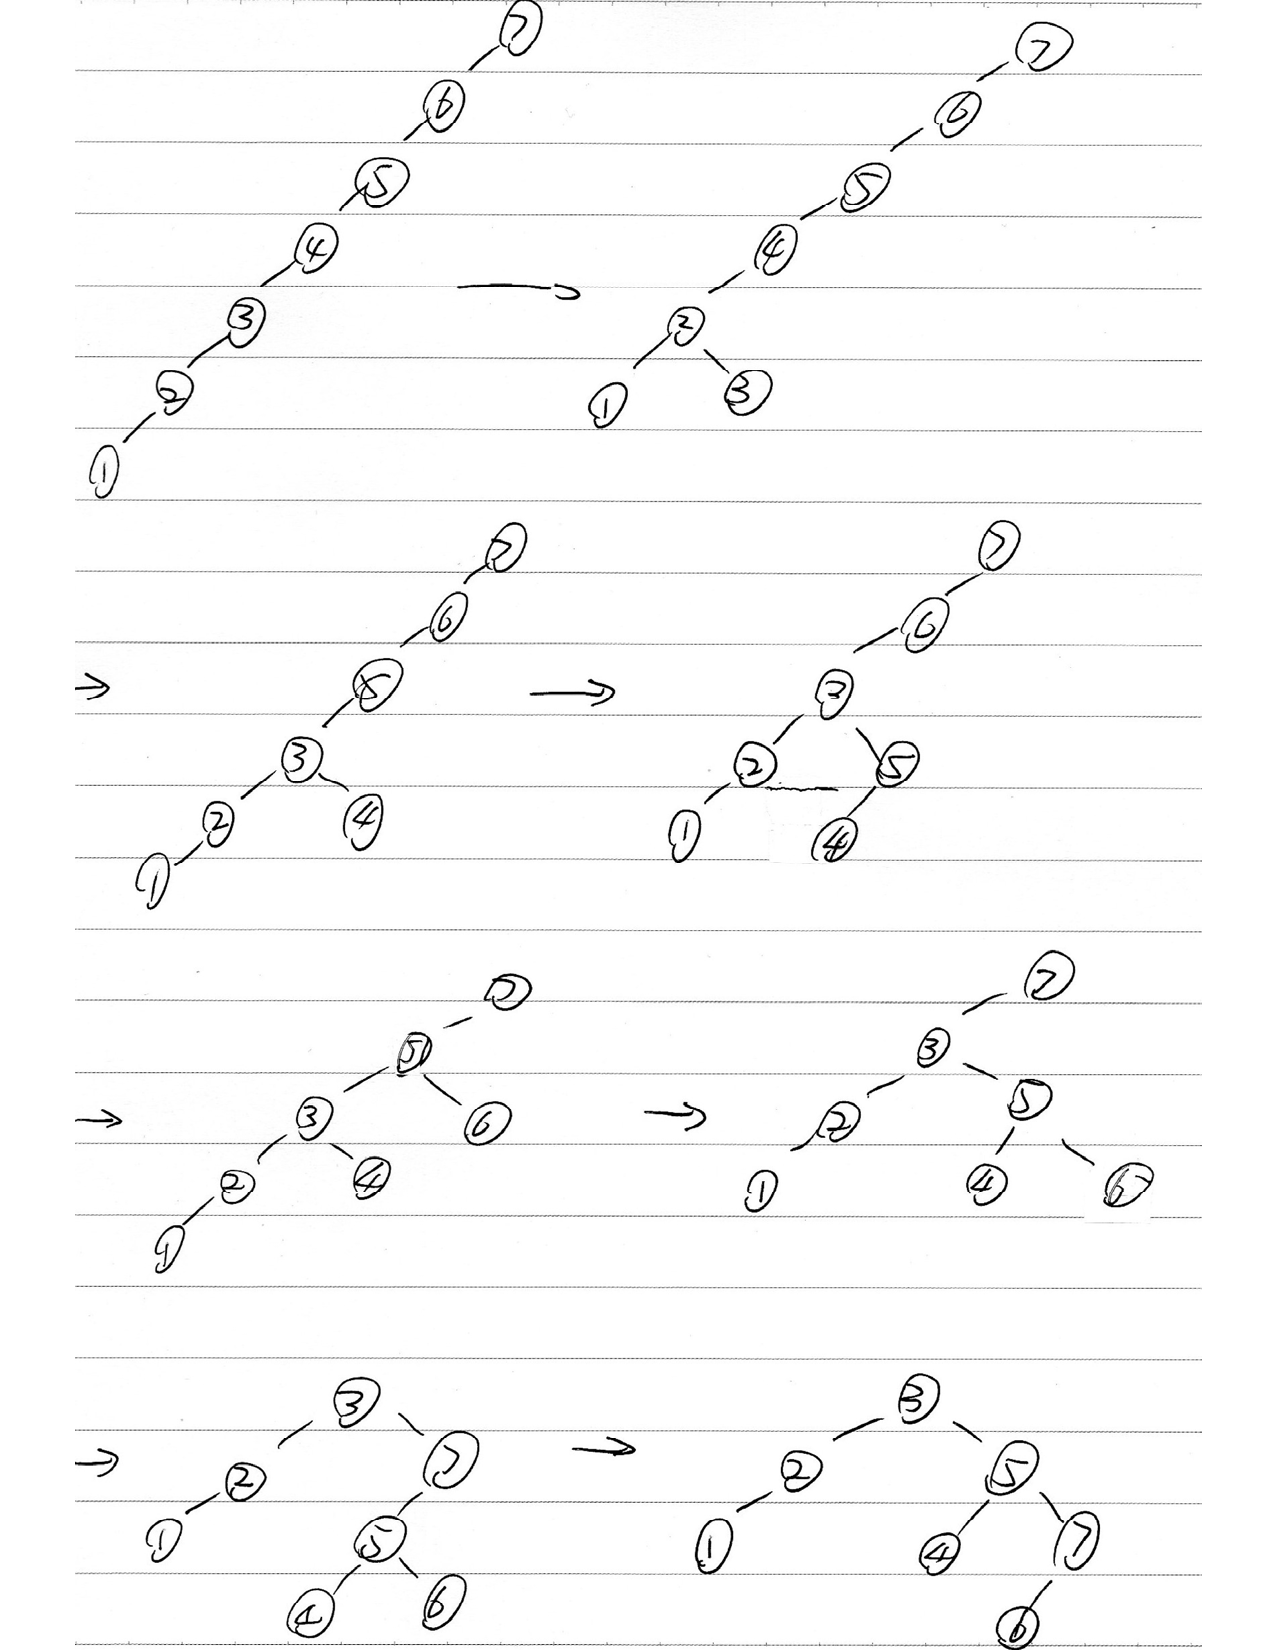
\includegraphics[width=\textwidth]{Pic/BST2AVL.pdf}
    \caption{Convert a BST to AVL}
  \end{figure}


\section*{Problem 3-3}
  \subsection*{(a)}
    If $H$ is strongly 2-universal, $\forall x_1 \neq x_2 \in U$, the distribution of $(h(x_1), h(x_2))$ is uniform distribution over plane $\mathbb{Z}^2$, thus
    $$ Pr(h(x_1) = h(x_2)) = \sum Pr((y, y)) = m / m^2 = \frac{1}{m}$$
  \subsection*{(b)}
    $$ U = \mathbb{Z}$$
    $$h_1(x) = x \mod 3$$
    $$h_2(x) = (x+1) \mod 3$$
    $$H = \{h_1, h_2\}$$
    \begin{center}\begin{table}[!hbp]
    \begin{tabular}{|c|c|c|c|c|c|c|}
      \hline
      $x$ & 1 & 2 & 3 & 4 & 5 & 6 \\ 
      \hline
      $h_1(x)$ & 1 & 2 & 0 & 1 & 2 & 0 \\
      \hline
      $h_2(x)$ & 2 & 0 & 1 & 2 & 0 & 1 \\
      \hline
      $h_1$, $h_2$ pair & (1,2) & (2,0) & (0,1) & (1,2) & (2,0) & (0,1) \\
      \hline
    \end{tabular}
    \end{table}\end{center}
    The probability for collision is $\frac{1}{m}$, but there will only be m pairs[3 pairs: (1, 2), (2, 0), (0, 1)] instead of $m^2$ pairs. Thus it can't be a strongly 2-universal.
  \subsection*{(c)}
    $$ U = \mathbb{Z}$$
    $$h_i(x) = (x+i) \mod m$$
    $$H = \{h_i | i \in [m]\}$$
    In this way, $\forall j \in [m]$, when given  $\forall x$, we can know $h_j(x)$, choose $y = x + m \neq x$, $h_j(y) = h_j(x)$, $Pr(h_j(y) = h_j(x)) = 1$

  \subsection*{(d)}
    Solve this by Bayes' Rule:
    $$Pr(h(y) = h(x) | h(x)) = \frac{Pr(h(x), h(y))}{Pr(h(x))} = \frac{\frac{1}{m^2}}{\frac{1}{m}} = \frac{1}{m}$$
    That is to say, for any $y$, the probability of collision is always $\frac{1}{m}$
\end{document}
